\chapter{Guided Waves and Cavities}\label{ch:b2:guided-waves}

A radar's pulse travels from the transmitter to the dish inside a
rectangular copper pipe; the light of an internet link travels ten
thousand kilometres inside a glass thread thinner than a hair; the
microwaves of an oven bounce between its walls and settle into a
pattern of hot and cold spots. A wave confined by conducting or
refracting walls is no longer a plane wave free to go anywhere: it
must satisfy the boundary conditions on the walls, and that selects
the shapes it may take --- the \emph{modes} --- and forbids it below a
\emph{cut-off} frequency. This chapter builds the simplest guide, two
parallel conducting plates, from the reflections of
\cref{ch:b2:wave-interfaces}; then the \omterm{prop:b2:guided-waves:rectangular}{rectangular waveguide}, the
closed cavity, and, in the ray picture, the \omterm{prop:b2:guided-waves:fibre}{optical fibre}.

\section{Waves between two conducting plates}

\begin{proposition}[Modes of the parallel-plate guide]\label{prop:b2:guided-waves:plates}
\index{waveguide}\index{guided wave}\index{mode (waveguide)}\index{cut-off frequency (waveguide)}
Two perfectly conducting planes $y = 0$ and $y = a$ bound a vacuum.
Seek a wave travelling along $z$ with $\vect E = E(y)\,\eu^{\iu(\omega t - k_gz)}
\vect e_x$ (the field parallel to the plates, perpendicular to the
propagation). \omterm{thm:b2:maxwell-equations:maxwell}{Maxwell's equations} in vacuum and the condition $E = 0$
on the plates impose
\[
E(y) = E_0\sin\frac{n\pi y}a , \qquad
k_g^2 = \frac{\omega^2}{c^2} - \Bigl(\frac{n\pi}a\Bigr)^2 , \qquad n = 1, 2, \dots
\]
Mode $n$ propagates only above its \emph{cut-off frequency} $f_n = nc/2a$;
below, $k_g$ is imaginary and the field decays along the guide. Its
phase and group velocities are
\[
v_\varphi = \frac c{\sqrt{1 - f_n^2/f^2}} > c , \qquad
v_g = c\sqrt{1 - f_n^2/f^2} < c , \qquad v_\varphi v_g = c^2 ,
\]
and its magnetic field has components along $y$ and along $z$: a
\omterm{prop:b2:guided-waves:plates}{guided wave} is not transverse in the direction of propagation.
\end{proposition}

\begin{proof}
Insert in $\Delta\vect E = \partial_t^2\vect E/c^2$: $E'' - k_g^2E = -(\omega^2/c^2)E$, i.e.\
$E'' + (\omega^2/c^2 - k_g^2)E = 0$, whose solutions vanishing at $y = 0$ and
$y = a$ are the sines with $\omega^2/c^2 - k_g^2 = (n\pi/a)^2$; $\operatorname{div}
\vect E = 0$ holds since $E_x$ does not depend on $x$. Faraday gives
$\underline B_y = (k_g/\omega)\underline E$ and $\underline B_z = (\iu/\omega)\partial_y\underline E$, the latter
in quadrature. The velocities follow from the Klein--Gordon form of
the \omterm{def:b2:dispersion-wave-packets:relation}{dispersion relation} (\cref{ch:b2:dispersion-wave-packets}).
\end{proof}

\begin{remark}[The mode as two plane waves]\label{rem:b2:guided-waves:zigzag}
$\sin(n\pi y/a)\eu^{-\iu k_gz}$ is the sum of two plane waves with
wavevectors $(0, \pm n\pi/a, k_g)$, of modulus $\omega/c$, bouncing between
the plates at the angle $\theta$ from the axis with $\cos\theta = k_gc/\omega$:
a guided mode is a plane wave zigzagging between the walls, reflected
with $r = -1$ at each one, the transverse \omterm{prop:b2:waves-on-strings:modes}{standing wave} being the
condition that it interferes constructively with itself. The energy
travels along the zigzag at $c$, hence along the axis at $c\cos\theta = v_g$;
the crests' intersections with the axis run at $c/\cos\theta = v_\varphi$. At
cut-off the wave bounces back and forth across the guide and goes
nowhere.
\end{remark}

\begin{omfigure}
\begin{tikzpicture}[font=\small, x=1cm, y=1cm, >=Stealth]
  \begin{scope}
    \draw[thick] (-3,0) -- (3,0); \draw[thick] (-3,2) -- (3,2);
    \fill[pattern=north east lines] (-3,-0.15) rectangle (3,0); \fill[pattern=north east lines] (-3,2) rectangle (3,2.15);
    \draw[omDef, thick, ->] (-2.8,0.2) -- (-1.6,1.8); \draw[omDef, thick, ->] (-1.6,1.8) -- (-0.4,0.2); \draw[omDef, thick, ->] (-0.4,0.2) -- (0.8,1.8); \draw[omDef, thick, ->] (0.8,1.8) -- (2.0,0.2); \draw[omDef, thick, ->] (2.0,0.2) -- (2.8,1.27);
    \draw (-0.4,0.2) -- (0.6,0.2); \draw (0.3,0.2) arc[start angle=0, end angle=53, radius=0.7]; \node[font=\footnotesize] at (0.75,0.55) {$\theta$};
    \draw[->, thick] (-3,-0.6) -- (3,-0.6) node[right, font=\footnotesize] {$z$};
    \node[font=\footnotesize] at (-3.3,1) {$a$};
    \draw[<->] (-3.15,0) -- (-3.15,2);
  \end{scope}
  \begin{scope}[xshift=8.4cm]
    \draw[thick] (0,0) -- (0,2); \draw[thick] (3.6,0) -- (3.6,2);
    \fill[pattern=north east lines] (-0.15,0) rectangle (0,2); \fill[pattern=north east lines] (3.6,0) rectangle (3.75,2);
    \draw[omThm, thick, domain=0:3.6, samples=50] plot (\x,{1+0.8*sin(50*\x)});
    \draw[omProp, thick, domain=0:3.6, samples=50] plot (\x,{1+0.6*sin(100*\x)});
    \draw[dashed] (0,1) -- (3.6,1);
    \node[omThm, font=\footnotesize] at (1.8,2.3) {$n = 1$}; \node[omProp, font=\footnotesize] at (0.9,1.9) {$n = 2$};
    \draw[<->] (0,-0.3) -- (3.6,-0.3) node[midway, below, font=\footnotesize] {$a$ (the $y$ axis)};
  \end{scope}
\end{tikzpicture}

{\small Left: a guided mode is a plane wave bouncing between the
plates; the angle $\theta$ opens as the frequency approaches cut-off.
Right: the transverse profiles $E(y)$ of the first two modes, vanishing
on the conducting walls.}
\end{omfigure}

\begin{omfigure}
\begin{tikzpicture}
\begin{axis}[omaxis, axis x line=bottom, axis y line=left, width=6.6cm, height=4.8cm,
    xlabel={$k_g$}, ylabel={$\omega$}, xmin=0, xmax=3, ymin=0, ymax=4, xtick=\empty, ytick={1,2,3}, yticklabels={$\omega_1$, $\omega_2$, $\omega_3$}, samples=80,
    xlabel style={at={(axis description cs:1.0,0.0)}, anchor=west},
    ylabel style={at={(axis description cs:0.0,1.0)}, anchor=south}]
  \addplot[omThm, thick, domain=0:3] {sqrt(1+x*x)};
  \addplot[omThm, thick, domain=0:3] {sqrt(4+x*x)};
  \addplot[omThm, thick, domain=0:3] {sqrt(9+x*x)};
  \addplot[omDef, dashed, domain=0:3] {x};
  \node[font=\scriptsize, anchor=west] at (axis cs:2.2,2.05) {$\omega = ck_g$};
\end{axis}
\end{tikzpicture}
\hfill
\begin{tikzpicture}
\begin{axis}[omaxis, axis x line=bottom, axis y line=left, width=6.6cm, height=4.8cm,
    xlabel={$f/f_1$}, ylabel={$v/c$}, xmin=1, xmax=4, ymin=0, ymax=2.5, xtick={1,2,3,4}, ytick={1}, samples=100,
    xlabel style={at={(axis description cs:0.5,-0.12)}, anchor=north},
    ylabel style={at={(axis description cs:-0.1,0.5)}, rotate=90, anchor=south},
    legend style={font=\scriptsize, at={(0.97,0.95)}, anchor=north east, draw=none, fill=none}]
  \addplot[omThm, thick, domain=1.05:4] {1/sqrt(1-1/(x*x))};
  \addplot[omDef, thick, domain=1:4] {sqrt(1-1/(x*x))};
  \addplot[black, dashed, domain=1:4] {1};
  \legend{$v_\varphi$, $v_g$}
\end{axis}
\end{tikzpicture}

{\small Left: the dispersion curves of the first three modes of a
guide, each a hyperbola starting at its cut-off. Right: phase and
group velocities of a mode against frequency; the energy crawls near
cut-off and approaches $c$ far above.}
\end{omfigure}

\begin{example}[Numbers]\label{ex:b2:guided-waves:numbers}
Plates \qty{3}{cm} apart: $f_1 = \qty{5}{GHz}$, $f_2 = \qty{10}{GHz}$; between
those frequencies only one mode propagates (\emph{single-mode}
operation, which keeps a pulse from splitting into several with
different $v_g$). At \qty{8}{GHz} the mode $n = 1$ has $v_g = 0.78c$, $v_\varphi =
1.28c$, and the guide wavelength $\lambda_g = 2\pi/k_g = \qty{4.8}{cm}$ instead of
\qty{3.75}{cm} in free space. At \qty{4}{GHz} nothing passes: the field
decays as $\eu^{-z/\ell}$ with $\ell = c/2\pi\sqrt{f_1^2 - f^2} = \qty{1.6}{cm}$ --- the
principle of the mesh in an oven door, of the waveguide below cut-off
used as a calibrated attenuator, and of the metal ducts of
ventilation that let air but no radio through.
\end{example}

\section{The rectangular waveguide and the cavity}

\begin{proposition}[The rectangular guide; the TE$_{10}$ mode]\label{prop:b2:guided-waves:rectangular}
\index{rectangular waveguide}\index{TE mode}
A hollow metal pipe of rectangular section $a \times b$ ($a > b$) carries
modes whose cut-off frequencies are
\[
f_{mn} = \frac c2\sqrt{\Bigl(\frac ma\Bigr)^2 + \Bigl(\frac nb\Bigr)^2} ;
\]
the lowest, the \emph{TE$_{10}$ mode} ($f_{10} = c/2a$), has $\vect E = E_0\sin
(\pi x/a)\,\eu^{\iu(\omega t - k_gz)}\,\vect e_y$: one half-sine across the wide
side, uniform across the narrow side, vanishing on the two walls $x = 0$,
$x = a$ --- exactly the parallel-plate mode, the side walls $y = 0$, $b$
being perpendicular to $\vect E$ and imposing nothing on it. The guide is
used between $f_{10}$ and the next cut-off; its magnetic field lines
close in the $xz$ plane and the currents they induce in the walls are
what a slot must not cut. The power carried is $\tfrac14\varepsilon_0cE_0^2\,ab
\sqrt{1 - f_{10}^2/f^2}$.
\end{proposition}

\begin{proof}
The general mode is $\cos$/$\sin$ products in $x$ and $y$ with the
boundary conditions on the four walls, giving $k_g^2 = \omega^2/c^2 - (m\pi/a)^2
- (n\pi/b)^2$ (admitted in general; the TE$_{10}$ case is the proposition
above). Power: the mean \omterm{thm:b2:poynting-vector:poynting}{Poynting vector} along $z$ is $E_0^2\sin^2(\pi x/a)
\,k_g/2\mu_0\omega$ integrated over the section.
\end{proof}

\begin{omfigure}
\begin{tikzpicture}[font=\small, x=1cm, y=1cm, >=Stealth]
  \begin{scope}
    \draw[thick] (0,0) rectangle (3.6,1.8);
    \foreach \x in {0.45,0.9,...,3.15} {
      \pgfmathsetmacro{\h}{0.75*sin(deg(180*\x/3.6))}
      \draw[omDef, ->] (\x,{0.9-\h}) -- (\x,{0.9+\h});
    }
    \node[font=\footnotesize] at (1.8,-0.35) {$a$}; \node[font=\footnotesize] at (-0.3,0.9) {$b$};
    \node[omDef, font=\footnotesize] at (1.8,2.15) {TE$_{10}$: $\vect E$ across the narrow side};
  \end{scope}
  \begin{scope}[xshift=7.0cm]
    \draw[thick] (0,0) rectangle (4.8,1.8);
    \draw[omProp, thick, postaction={decorate, decoration={markings, mark=at position 0.2 with {\arrow{>}}, mark=at position 0.7 with {\arrow{>}}}}] (1.2,0.9) ellipse (0.9 and 0.55);
    \draw[omProp, thick, postaction={decorate, decoration={markings, mark=at position 0.2 with {\arrow{<}}, mark=at position 0.7 with {\arrow{<}}}}] (3.6,0.9) ellipse (0.9 and 0.55);
    \node[omProp, font=\footnotesize] at (2.4,2.15) {$\vect B$ loops in the $xz$ plane (top view)};
    \draw[->, thick] (0,-0.85) -- (1.2,-0.85) node[right, font=\footnotesize] {$z$};
    \draw[<->] (0,-0.3) -- (2.4,-0.3) node[midway, below, font=\footnotesize] {$\lambda_g/2$};
  \end{scope}
\end{tikzpicture}

{\small The TE$_{10}$ mode of a rectangular guide: the electric field
spans the narrow dimension with a half-sine profile across the wide
one; the magnetic field closes in loops in the plane of the wide
faces, a half guide wavelength long.}
\end{omfigure}

\begin{proposition}[Cavity resonator]\label{prop:b2:guided-waves:cavity}
\index{cavity resonator}\index{mode (cavity)}
Closing a guide with two conducting walls a length $d$ apart turns it
into a \emph{cavity}, in which the \omterm{prop:b2:guided-waves:plates}{guided wave} must form a \omterm{prop:b2:waves-on-strings:modes}{standing
wave} along $z$ too: $k_g = p\pi/d$, and the resonance frequencies of a
rectangular box $a \times b \times d$ are
\[
f_{mnp} = \frac c2\sqrt{\Bigl(\frac ma\Bigr)^2 + \Bigl(\frac nb\Bigr)^2 + \Bigl(\frac pd\Bigr)^2} .
\]
The number of modes with frequency below $f$ grows as $8\pi V f^3/3c^3$ for
a box of volume $V$ (admitted: count the points of the lattice
$(m/2a, n/2b, p/2d)$ in an eighth of a sphere, with two polarizations)
--- the density of modes that the theory of thermal radiation will
need (\cref{ch:b2:thermal-radiation}). Each mode has a quality factor
$Q$ set by the wall losses (the surface resistance of
\cref{ch:b2:waves-in-media}), typically $10^3$--$10^4$ for copper at
microwave frequencies, $10^{10}$ for a superconducting cavity.
\end{proposition}

\begin{proof}
\omterm{prop:b2:waves-on-strings:modes}{Standing waves} along the three directions with nodes on the six walls;
the wavevector $(m\pi/a, n\pi/b, p\pi/d)$ has modulus $\omega/c$.
\end{proof}

\begin{example}[Ovens, radars, clocks]\label{ex:b2:guided-waves:cavities}
A microwave oven of $30 \times 30 \times 20$ cm$^3$ near \qty{2.45}{GHz} has
dozens of modes within a few percent of the magnetron's frequency:
the field is a superposition of \omterm{prop:b2:waves-on-strings:modes}{standing waves}, with maxima
\qty{6}{cm} apart, which the turntable (and a "mode stirrer") smooth
out. A radar's magnetron is itself a \omterm{prop:b2:guided-waves:cavity}{cavity resonator}; a particle
accelerator is a chain of superconducting cavities whose TM mode
pushes the bunches; the atoms of a caesium clock cross a microwave
cavity tuned to \qty{9.19}{GHz}.
\end{example}

\section{The optical fibre in the ray picture}

\begin{proposition}[Step-index fibre]\label{prop:b2:guided-waves:fibre}
\index{optical fibre}\index{numerical aperture}\index{modal dispersion}
A glass core of index $n_1$ surrounded by a cladding of slightly lower
index $n_2$ guides light by \omterm{thm:b2:wave-interfaces:snell}{total internal reflection} at the core
boundary. A ray entering the end face from air at the angle $\alpha$ from
the axis is trapped if $\sin\alpha < \sqrt{n_1^2 - n_2^2}$, the \emph{\omterm{prop:b2:guided-waves:fibre}{numerical
aperture}}; rays of different angles travel different lengths, and a
pulse entering a fibre of length $L$ is spread by
\[
\Delta t = \frac{n_1L}c\Bigl(\frac{n_1}{n_2} - 1\Bigr) ,
\]
the \emph{\omterm{prop:b2:guided-waves:fibre}{modal dispersion}} --- some \qty{50}{ns} per kilometre for $n_1
- n_2 = 0.01$, which limits a multimode fibre to a few megabits per
second over ten kilometres. A \emph{single-mode} fibre has a core so
thin (\qty{9}{\micro m}) that only one mode propagates, like the guide
between its first two cut-offs; what remains is the chromatic
dispersion of the glass (\cref{ch:b2:dispersion-wave-packets}).
\end{proposition}

\begin{proof}
Total reflection at the core--cladding interface needs $\sin\theta >
n_2/n_1$ for the angle $\theta$ from the normal to the boundary, i.e.\ $\cos
\theta' > n_2/n_1$ for the angle $\theta'$ from the axis inside; refraction
at the entrance gives $\sin\alpha = n_1\sin\theta'$, whence $\sin\alpha < n_1\sqrt{1
- n_2^2/n_1^2}$. The steepest trapped ray travels $L/\cos\theta' = Ln_1/n_2$
against $L$ for the axial one, at $c/n_1$.
\end{proof}

\begin{omfigure}
\begin{tikzpicture}[font=\small, x=1cm, y=1cm, >=Stealth]
  \fill[omDef!10] (-3.5,-1.0) rectangle (3.5,1.0);
  \fill[omDef!30] (-3.5,-0.5) rectangle (3.5,0.5);
  \draw[thick] (-3.5,0.5) -- (3.5,0.5) (-3.5,-0.5) -- (3.5,-0.5);
  \draw[omThm, thick, ->] (-4.6,-0.9) -- (-3.5,-0.35);
  \draw[omThm, thick] (-3.5,-0.35) -- (-2.3,0.5) -- (-0.9,-0.5) -- (0.5,0.5) -- (1.9,-0.5) -- (3.3,0.5);
  \draw[omProp, thick, ->] (-4.6,0) -- (3.4,0);
  \draw[dashed] (-3.5,-1.3) -- (-3.5,1.3);
  \node[font=\footnotesize] at (-4.3,-0.25) {$\alpha$};
  \node[font=\footnotesize] at (2.6,0.8) {cladding $n_2$}; \node[font=\footnotesize] at (2.6,0.2) {core $n_1$};
  \node[font=\footnotesize] at (0,-1.4) {$\sin\alpha < \sqrt{n_1^2 - n_2^2}$: trapped by total internal reflection};
\end{tikzpicture}

{\small A step-index fibre in the ray picture: rays within the
acceptance cone are trapped by \omterm{thm:b2:wave-interfaces:snell}{total internal reflection}; the zigzag
ray arrives after the axial one --- \omterm{prop:b2:guided-waves:fibre}{modal dispersion}.}
\end{omfigure}

\begin{method}[Guided-wave bookkeeping]\label{met:b2:guided-waves:method}
(1) Identify the walls and their condition (tangential $\vect E = 0$ on
a conductor; total reflection for a dielectric). (2) Write the field
as a transverse \omterm{prop:b2:waves-on-strings:modes}{standing wave} times a progressive factor along the
guide; the boundary conditions quantize the transverse wavenumber.
(3) The \omterm{def:b2:dispersion-wave-packets:relation}{dispersion relation} $k_g^2 = \omega^2/c^2 - k_\perp^2$ gives the
cut-off, $v_\varphi$, $v_g$, $\lambda_g$. (4) Count the propagating modes at the
working frequency; aim for one. (5) For a cavity add the longitudinal
condition and find the resonance frequencies; for the losses use the
surface resistance.
\end{method}

\section{Exercises}

\begin{exercise}[$\star$]\label{exo:b2:guided-waves:1}
Plates \qty{2.0}{cm} apart: cut-off frequencies of the first three modes;
at \qty{12}{GHz}, which modes propagate, and for the first one $k_g$,
$\lambda_g$, $v_\varphi$, $v_g$; at \qty{6}{GHz}, the decay length of the field.
\end{exercise}

\begin{exercise}[$\star$]\label{exo:b2:guided-waves:2}
A standard X-band waveguide has $a = \qty{22.9}{mm}$, $b = \qty{10.2}{mm}$.
Cut-off of TE$_{10}$, of TE$_{20}$ and TE$_{01}$; the single-mode band; at
\qty{10}{GHz}: $\lambda_g$, $v_g$, the angle of the zigzag. Why is $b \approx a/2$
a good choice?
\end{exercise}

\begin{exercise}[$\star$]\label{exo:b2:guided-waves:3}
A cavity of $30 \times 30 \times 20$ cm$^3$: frequencies of the modes $(1,1,0)$,
$(1,0,1)$, $(2,1,1)$, $(3,2,1)$; number of modes below \qty{2.5}{GHz} from
the counting formula; the lowest mode of a \qty{9.19}{GHz} cubic cavity
--- its side.
\end{exercise}

\begin{exercise}[$\star$]\label{exo:b2:guided-waves:4}
A fibre has $n_1 = 1.48$, $n_2 = 1.46$. \omterm{prop:b2:guided-waves:fibre}{Numerical aperture} and acceptance
half-angle; modal spread per kilometre; maximum bit rate over
\qty{2}{km} if one bit must last longer than the spread; the same with
$n_1 - n_2 = 0.003$.
\end{exercise}

\begin{exercise}[$\star\star$]\label{exo:b2:guided-waves:5}
For the parallel-plate mode $n = 1$: (a) find $\vect B$ from Faraday's
law and show it has a $z$ component in quadrature with $E$. (b) \omterm{prop:b2:maxwell-equations:boundary}{Surface
current} on each plate (boundary relation). (c) Mean \omterm{thm:b2:poynting-vector:poynting}{Poynting vector}
along $z$ and the power per unit width; check that its transverse
component averages to zero. (d) Show that the energy velocity, power
over mean energy per unit length, equals $v_g$.
\end{exercise}

\begin{exercise}[$\star\star$]\label{exo:b2:guided-waves:6}
\emph{Below cut-off.} (a) A \qty{1}{mm} hole in the \qty{0.5}{mm} mesh of an
oven door at \qty{2.45}{GHz}: treat it as a guide of width $a = \qty{1}{mm}$;
decay length and \omterm{def:b2:dispersion-wave-packets:complex}{attenuation} across the sheet in dB (compare
\cref{ch:b2:waves-in-media}). (b) A ventilation duct of \qty{20}{cm}
section in a shielded room: up to what frequency does it block radio,
and by how much does it attenuate \qty{100}{MHz} over \qty{1}{m}? (c) A
"waveguide-beyond-cutoff attenuator" uses a tube of \qty{1}{cm} diameter at
\qty{1}{GHz}: \omterm{def:b2:dispersion-wave-packets:complex}{attenuation} per centimetre (use the plate formula with $a =
\qty{1}{cm}$ as an estimate). (d) Why is the \omterm{def:b2:dispersion-wave-packets:complex}{attenuation} independent of
the wall conductivity?
\end{exercise}

\begin{exercise}[$\star\star$]\label{exo:b2:guided-waves:7}
\emph{Power and breakdown.} The X-band guide of \cref{exo:b2:guided-waves:2}
carries TE$_{10}$ at \qty{10}{GHz}. (a) Power for $E_0 = \qty{1}{MV/m}$. (b) Air
breaks down at \qty{3}{MV/m}: maximum power; how do radars carry
megawatts (pressurization, gases)? (c) Wall losses: the \omterm{prop:b2:maxwell-equations:boundary}{surface current}
at the broad wall is of order $E_0/\mu_0c$; with $R_s = \qty{0.026}{\ohm}$ for
copper at \qty{10}{GHz}, estimate the loss per metre and the \omterm{def:b2:dispersion-wave-packets:complex}{attenuation}
in dB/m. (d) Compare with a \omterm{prop:b2:dispersion-wave-packets:coax}{coaxial cable}'s \qty{0.5}{dB/m}: why are
guides used at these frequencies?
\end{exercise}

\begin{exercise}[$\star\star$]\label{exo:b2:guided-waves:8}
\emph{Cavity quality.} A copper cubic cavity of side \qty{10}{cm} in its
lowest mode. (a) Frequency. (b) The stored energy is $\tfrac12\varepsilon_0E_0^2V/4$
(admitted) and the wall loss $\tfrac12R_sH_0^2\times$ area with $H_0 \approx E_0/
\mu_0c$ and $R_s = 1/\gamma\delta$: quality factor $Q = \omega W/P$ --- compute it.
(c) Bandwidth $f/Q$ of the resonance; ring-down time $Q/\omega$. (d) A
superconducting cavity has $R_s \sim \qty{1e-8}{\ohm}$: $Q$, and why
accelerators use them.
\end{exercise}

\begin{exercise}[$\star\star$]\label{exo:b2:guided-waves:9}
\emph{Mode counting.} (a) Show that the number of modes of a box of
volume $V$ with frequency below $f$ is $N(f) = 8\pi Vf^3/3c^3$ (points
$(m, n, p)$ in the eighth of a sphere of radius $2fL/c$ for a cube, two
polarizations). (b) The number of modes per unit volume and frequency,
$\dd N/V\dd f = 8\pi f^2/c^3$. (c) A \qty{1}{m^3} room: modes per hertz at
\qty{1}{GHz}; at \qty{500}{THz} (visible light). (d) Why does a small
cavity have sparse modes while a big room has a continuum --- and what
is the oven's case at \qty{2.45}{GHz}?
\end{exercise}

\begin{exercise}[$\star\star\star$]\label{exo:b2:guided-waves:10}
\emph{TE$_{10}$ in full.} In the guide $0 < x < a$, $0 < y < b$: $\vect E =
E_0\sin(\pi x/a)\eu^{\iu(\omega t - k_gz)}\vect e_y$. (a) From Faraday, find $\underline B_x$
and $\underline B_z$; check $\operatorname{div}\vect B = 0$. (b) Check Maxwell--Ampère
in vacuum, and recover $k_g^2 = \omega^2/c^2 - (\pi/a)^2$. (c) \omterm{prop:b2:maxwell-equations:boundary}{Surface currents}
on the four walls (the broad walls $y = 0$, $b$ and the narrow walls $x = 0$,
$a$); which currents flow along $z$, which across? (d) A slot cut along
$z$ in the centre of a broad wall does not radiate, a slot across it
does: explain.
\end{exercise}

\begin{exercise}[$\star\star\star$]\label{exo:b2:guided-waves:11}
\emph{Dielectric guide.} A slab of index $n_1$ and thickness $a$ in a
medium $n_2 < n_1$ guides light by total reflection. (a) For a ray at
angle $\theta$ from the normal to the faces, the guided condition is that
the round-trip phase across the slab, $2k_0n_1a\cos\theta - 2\varphi_r$ ($\varphi_r$
the phase shift of total reflection, taken $\approx 0$ here), is a multiple
of $2\pi$: number of modes for $a = \qty{50}{\micro m}$, $\lambda = \qty{1.5}{\micro m}$,
$n_1 = 1.48$, $n_2 = 1.46$ (admit the mode count $\approx 2a\sqrt{n_1^2 - n_2^2}/\lambda$
per polarization). (b) Thickness for a single mode. (c) Compare with a
single-mode fibre core of \qty{9}{\micro m}. (d) Why can the dielectric
guide, unlike the metal one, not have a cut-off for its lowest mode?
\end{exercise}

\begin{exercise}[$\star\star\star$]\label{exo:b2:guided-waves:12}
\emph{Graded-index fibre.} To reduce \omterm{prop:b2:guided-waves:fibre}{modal dispersion} the core index
decreases from the axis outward, $n(r) = n_1\sqrt{1 - 2\Delta(r/a)^2}$ with
$\Delta \approx 0.01$. (a) Explain qualitatively why an off-axis ray, though
longer, can take the same time as the axial one. (b) Using the ray
equation in a stratified medium, $n(r)\cos\theta(r) = $ const, show that
a ray launched from the axis at a small angle oscillates sinusoidally
about it (expand $n$ to second order). (c) Period of the oscillation
for $a = \qty{25}{\micro m}$. (d) The residual modal spread is of order
$n_1L\Delta^2/2c$: value per kilometre, compared with the step-index
$n_1L\Delta/c$.
\end{exercise}

\begin{omfigure}
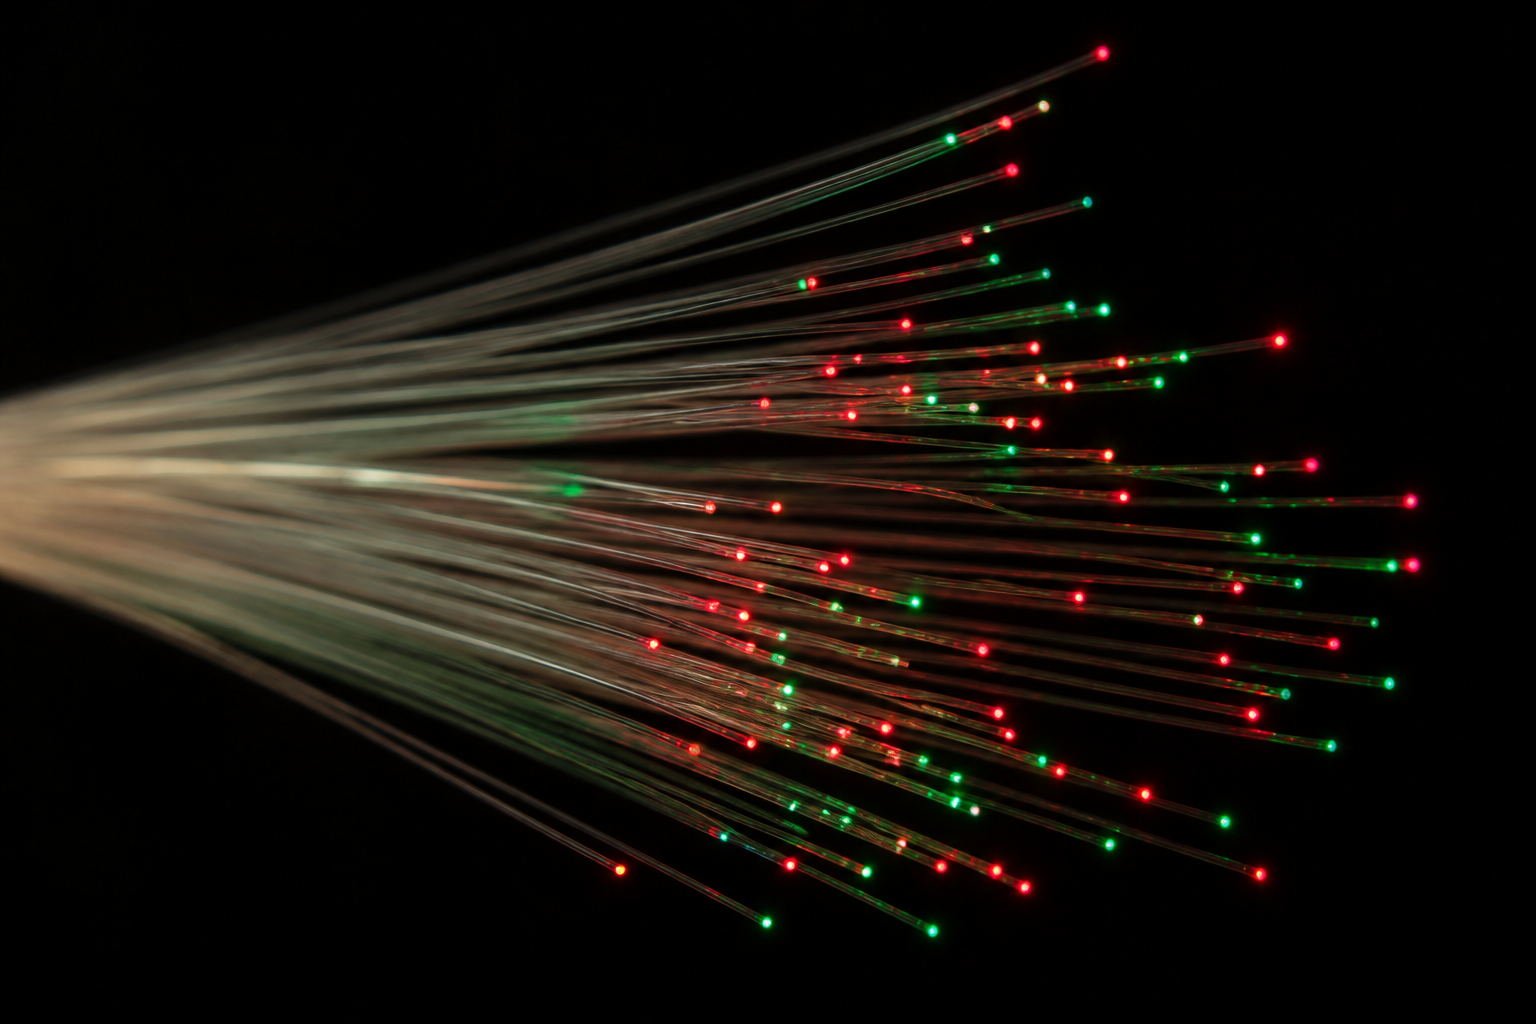
\includegraphics[width=0.58\linewidth]{images/book4/ai/b4-16-optical-fibres-glow.png}

{\small \omterm{prop:b2:guided-waves:fibre}{Optical fibres} lit from their far ends: light trapped by \omterm{thm:b2:wave-interfaces:snell}{total internal reflection} in a core thinner than a hair, and guided round every gentle bend.}
\end{omfigure}

\section{Problem: The oven cavity and the optical fibre}

\begin{problem}[{Weekend problem --- two guided-wave systems in every
kitchen and every city: the oven that cooks with standing waves and
the fibre that carries the internet}]
\label{pb:b2:guided-waves:1}

\medskip
\noindent\textbf{Part I --- From the magnetron to the cavity.}
A magnetron feeds \qty{800}{W} at \qty{2.45}{GHz} into a \omterm{prop:b2:guided-waves:rectangular}{rectangular
waveguide} ($a = \qty{8.6}{cm}$, $b = \qty{4.3}{cm}$) that opens into the oven
cavity ($30 \times 30 \times 20$ cm$^3$); walls steel, $\gamma = \qty{1e6}{S/m}$.
\begin{enumerate}
  \item Cut-off frequencies of the guide's TE$_{10}$, TE$_{20}$, TE$_{01}$
        modes; check that only TE$_{10}$ propagates at \qty{2.45}{GHz}.
  \item Guide wavelength, phase and group velocities at \qty{2.45}{GHz}.
  \item Field amplitude $E_0$ in the guide for \qty{800}{W} (TE$_{10}$ power
        formula); compare with the breakdown field of air.
  \item \omterm{prop:b2:maxwell-equations:boundary}{Surface current} amplitude on the broad wall (of order
        $E_0/\mu_0c$); \omterm{def:b2:dispersion-wave-packets:complex}{skin depth} and surface resistance of the steel;
        loss per metre of guide.
  \item Modes of the cavity: list those with frequencies within $3\%$
        of \qty{2.45}{GHz} (try $(m, n, p)$ up to $4$); how many?
  \item Distance between the hot spots of one such mode along each
        axis; why does the plate turn, and what is a "mode stirrer"?
  \item The cavity's quality factor when loaded with food is about
        $200$: bandwidth of its response; why a mismatch between the
        magnetron's frequency and the modes does not matter much.
  \item The empty cavity has $Q \approx 3000$: stored energy at \qty{800}{W}
        input, mean energy density, field amplitude; compare with
        question 3 and with breakdown. What protects the magnetron
        when the oven runs empty?
  \item Time for the energy to travel the \qty{20}{cm} of guide from
        the magnetron to the cavity.
  \item The magnetron is fed by a half-wave rectified supply and emits
        only during half of each mains cycle: peak power during the
        bursts for a mean of \qty{800}{W}; what does the cavity do
        between bursts (use $Q \approx 200$)?
\end{enumerate}

\medskip
\noindent\textbf{Part II --- The door and the cut-off.}
\begin{enumerate}[resume]
  \item The door mesh has \qty{1.5}{mm} holes in a \qty{1}{mm} sheet: decay
        length in a hole and \omterm{def:b2:dispersion-wave-packets:complex}{attenuation} in dB across the sheet.
  \item The door's edge is sealed by a quarter-wave "choke": a slot
        $\lambda/4$ deep around the door frame, which presents an open
        circuit at the gap (recall \cref{ch:b2:wave-interfaces}): depth
        of the slot at \qty{2.45}{GHz}.
  \item Legal leakage is \qty{5}{mW/cm^2} at \qty{5}{cm}: to what fraction of
        \qty{800}{W} through a \qty{100}{cm^2} door does that correspond?
  \item A \qty{30}{cm} duct of \qty{4}{cm} diameter vents the cavity: is it
        below cut-off at \qty{2.45}{GHz}? \omterm{def:b2:dispersion-wave-packets:complex}{Attenuation} over its length.
  \item Why must the mesh be electrically bonded to the door frame all
        round (what would a gap in the bond behave like)?
\end{enumerate}

\medskip
\noindent\textbf{Part III --- The fibre.}
A step-index fibre: core $n_1 = 1.465$, cladding $n_2 = 1.460$, core
diameter \qty{50}{\micro m} (multimode) or \qty{9}{\micro m} (single-mode);
$\lambda = \qty{1.55}{\micro m}$; \omterm{def:b2:dispersion-wave-packets:complex}{attenuation} \qty{0.2}{dB/km}.
\begin{enumerate}[resume]
  \item \omterm{prop:b2:guided-waves:fibre}{Numerical aperture} and acceptance angle; is it easy to couple
        light in?
  \item Modal spread per kilometre for the multimode fibre; maximum
        bit rate over \qty{10}{km} (one bit per spread time).
  \item Number of modes of the multimode fibre (admit $N \approx
        \tfrac12(\pi d\,\mathrm{NA}/\lambda)^2$); of the single-mode one ($d =
        \qty{9}{\micro m}$: show the same formula gives about $1$).
  \item In the single-mode fibre the remaining spreading is chromatic:
        with $\omega'' \approx \qty{-0.2}{m^2/s}$ (\cref{ch:b2:dispersion-wave-packets})
        and \qty{50}{ps} pulses, distance over which a pulse doubles;
        bit rate over \qty{100}{km}.
  \item \omterm{def:b2:dispersion-wave-packets:complex}{Attenuation} over \qty{100}{km} in dB and as a power ratio; input
        \qty{1}{mW}: output power; with amplifiers every \qty{80}{km}, how
        many for a \qty{6000}{km} transatlantic link?
  \item Frequency and photon energy at \qty{1.55}{\micro m}; photons per
        second in \qty{1}{mW}, and per bit at \qty{10}{Gbit/s}, at the input
        and after \qty{100}{km}.
  \item Why \qty{1.55}{\micro m} (think of the two loss mechanisms of
        silica: Rayleigh scattering, falling as $1/\lambda^4$, and infrared
        absorption rising beyond \qty{1.6}{\micro m})?
  \item Fresnel reflection at a cleaved fibre end facing air: loss in
        dB; why connectors use index-matching gel or polished physical
        contact.
  \item Why does a fibre not radiate at a gentle bend, and why does
        it lose light at a sharp one (think of the angle of the ray
        on the core boundary)?
  \item Compare the two guides of this problem: what confines the
        wave, what limits the bandwidth, what the losses.
\end{enumerate}
\end{problem}
